\documentclass{article}
\usepackage[italian]{babel}
\usepackage[utf8]{inputenc}
\usepackage{fancyhdr}
\usepackage{tikz}
\usepackage{float}
\usepackage{amsmath}
\usepackage{amssymb}
\usepackage{amsthm}
\usepackage{amsfonts}
\usepackage{color}
\usepackage{circuitikz}
\usepackage[margin=2cm]{geometry}
\usepackage[scientific-notation=true]{siunitx}
\usepackage{titlesec}
\usepackage{graphics}

\titleformat{\paragraph}
  {\normalfont\normalsize\bfseries}{\theparagraph}{1em}{}
\titlespacing*{\paragraph}
  {0pt}{3.25ex plus 1ex minus .2ex}{1.5ex plus .2ex}

\title{Misura della caratteristica di due diodi a giunzione p-n}
\date{Quarto turno}
\author{Bertasi Leonardo, Perniola Davide }
\begin{document}
\maketitle
\section{Introduzione} 
Una giunzione p-n è composta da due regioni con drogaggio differente, di tipo p e di tipo n, di un semiconduttore a contatto tra di loro. Quando ai suoi capi è applicato una differenza di potenziale si parla di diodo. 
La prova è consistita nel misurare la caratteristica I-V di due diodi a semiconduttore, uno al silicio e uno al germanio, con l'obiettivo di ricavare il valore della corrente inversa $I_0$ e del prodotto $\eta V_T$ ($\eta$ fattore di idealità, $V_T$ equivalemte in volt della temperatura della giunzione).
Sono stati utilizzati, inoltre, un alimentatore di bassa tensione, un multimetro digitale, un oscilloscopio, un potenziometro da $1k\Omega$ oltre che dai due diodi in esame.
Il circuito realizzato è riporato in Figura 1.
\vspace{0.5cm}

\begin{figure}[H]
  \centering
  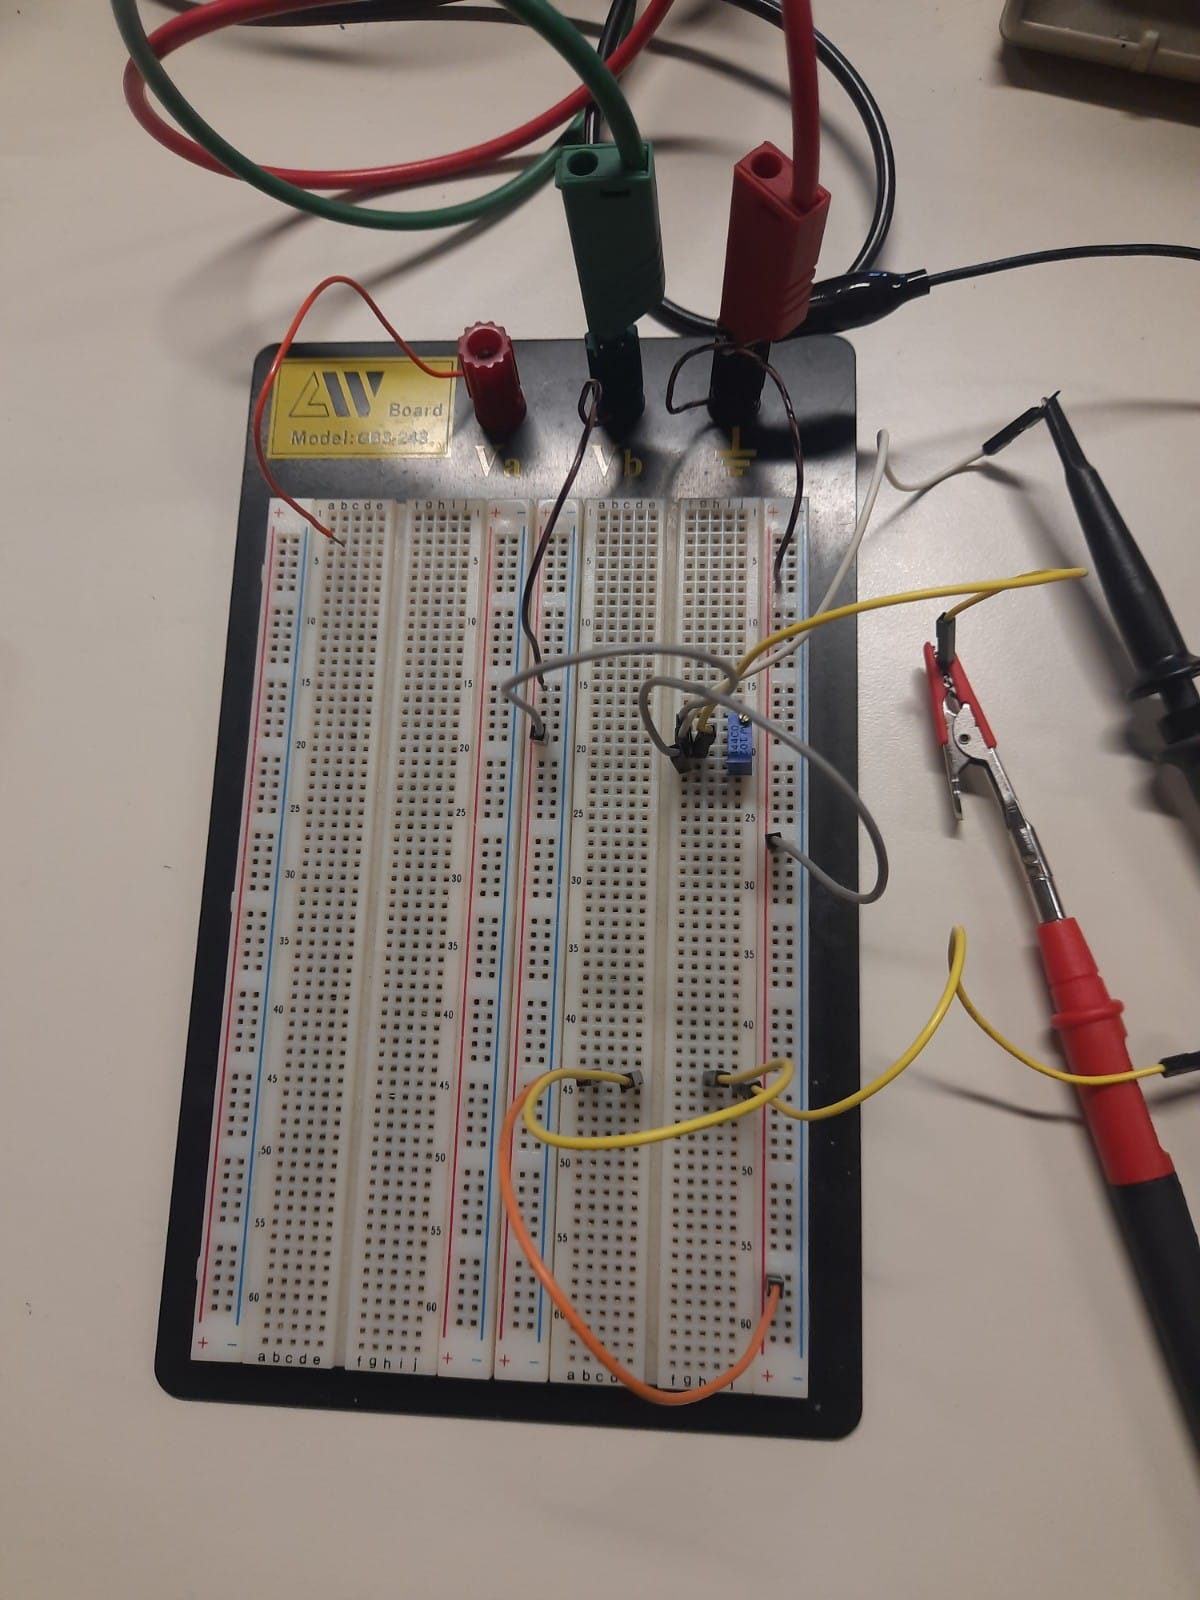
\includegraphics[scale=0.11]{Diod.jpg}
  \qquad
  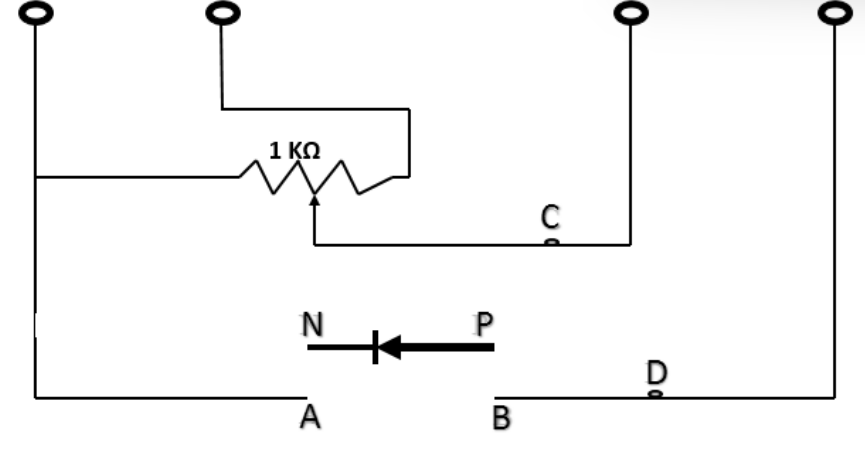
\includegraphics[scale=0.55]{Circ1.png}
  \qquad
  \caption{\textit{Circuito realizzato e una sua rappresentazione schematica. }}
\end{figure}


\section{Risultati}
In Tabella 1 e 2 sono riportati i valori misurati di $I$ e $V$ utilizzati per i fit in Figura 2 e 3. Gli errori sui valori misurati con l'oscilloscopio sono stati ricavati considerando la somma quadratica dell'errore sulla lettura, sullo zero e del costruttore, secondo la relazione\\
\\
$\sigma = \sqrt{(\sigma_L+\sigma_Z)^2+\sigma_C^2} $\\


\begin{table}[h!]
  \centering
 \mbox{%
\begin{tabular}{|c|c|c|}

\hline
$F.S(mV/div)$ & $V(mV)$ & $I(mA)$\\
\hline

$100$ & $665\pm{22}$ & $1.74\pm{0.04}$ \\
$100$ & $650\pm{22}$ & $1.50\pm{0.03}$ \\
$100$ & $645\pm{22}$ & $1.25\pm{0.03}$ \\
$100$ & $635\pm{22}$ & $0.98\pm{0.02}$ \\
$100$ & $625\pm{21}$ & $0.69\pm{0.02}$ \\
$100$ & $605\pm{21}$ & $0.53\pm{0.02}$ \\
$100$ & $590\pm{20}$ & $0.36\pm{0.02}$ \\
$100$ & $565\pm{20}$ & $0.22\pm{0.01}$ \\
$100$ & $525\pm{19}$ & $0.10\pm{0.01}$ \\
$100$ & $500\pm{18}$ & $0.05\pm{0.01}$ \\
$100$ & $445\pm{17}$ & $0.02\pm{0.01}$ \\
$100$ & $430\pm{16}$ & $0.01\pm{0.01}$ \\

\hline
\end{tabular}
 }
 \caption{\textit{Risultati delle misure effettuate con il diodo al silicio e utilizzate per il fit. Sono riportate i valori di corrente e delle differenze di potenziale corrispettive, oltre che il fondo scale scelto per ogni misura}}
 \vspace{1cm}

\end{table}


\begin{table}[h!]
  \centering
 \mbox{%
\begin{tabular}{|c|c|c|}

\hline
$F.S(mV/div)$ & $V(mV)$ & $I(mA)$\\
\hline

$50$ & $285\pm{10}$ & $1.28\pm{0.03}$ \\
$50$ & $275\pm{10}$ & $1.01\pm{0.03}$ \\
$50$ & $255\pm{9}$ & $0.73\pm{0.02}$ \\
$50$ & $245\pm{9}$ & $0.58\pm{0.02}$ \\
$50$ & $225\pm{8}$ & $0.42\pm{0.02}$ \\
$50$ & $212\pm{8}$ & $0.32\pm{0.01}$ \\
$50$ & $182\pm{7}$ & $0.18\pm{0.01}$ \\
$50$ & $155\pm{7}$ & $0.10\pm{0.01}$ \\
$50$ & $135\pm{6}$ & $0.06\pm{0.01}$ \\
$20$ & $100\pm{4}$ & $0.02\pm{0.01}$ \\
$20$ & $85\pm{3}$ & $0.01\pm{0.01}$ \\

\hline
\end{tabular}
 }
 \caption{\textit{Risultati delle misure effettuate con il diodo al germanio e utilizzate per il fit. Sono riportate i valori di corrente e delle differenze di potenziale corrispettive, oltre che il fondo scale scelto per ogni misura}}
\end{table}
Considerando i grafici, il parametro $p_1$ rappresente il valore di $\eta V_T$ mentre $p_0=\eta V_T\ln{I_0}$. Risulta allora che per il diodo al silicio \\
\\
$I_0 = (1,07\pm1.20)nA $ \\
\\
$\eta V_T = (46.26\pm3.21)mV $  \\
\\
\\
e per il diodo al germanio \\
\\
$I_0 = (1.36\pm0.36)\mu A $ \\
\\
$\eta V_T = (39.28\pm1.07)mV $ \\
\\
C'è da considerare che gli errori sui valori della corrente inversa $I_0$ sono stati calcolati propagando le incertezze sui valori di $p_0$ e $p_1$ e sono da considerarsi come errori massimi.


\begin{figure}[H]
  \centering
  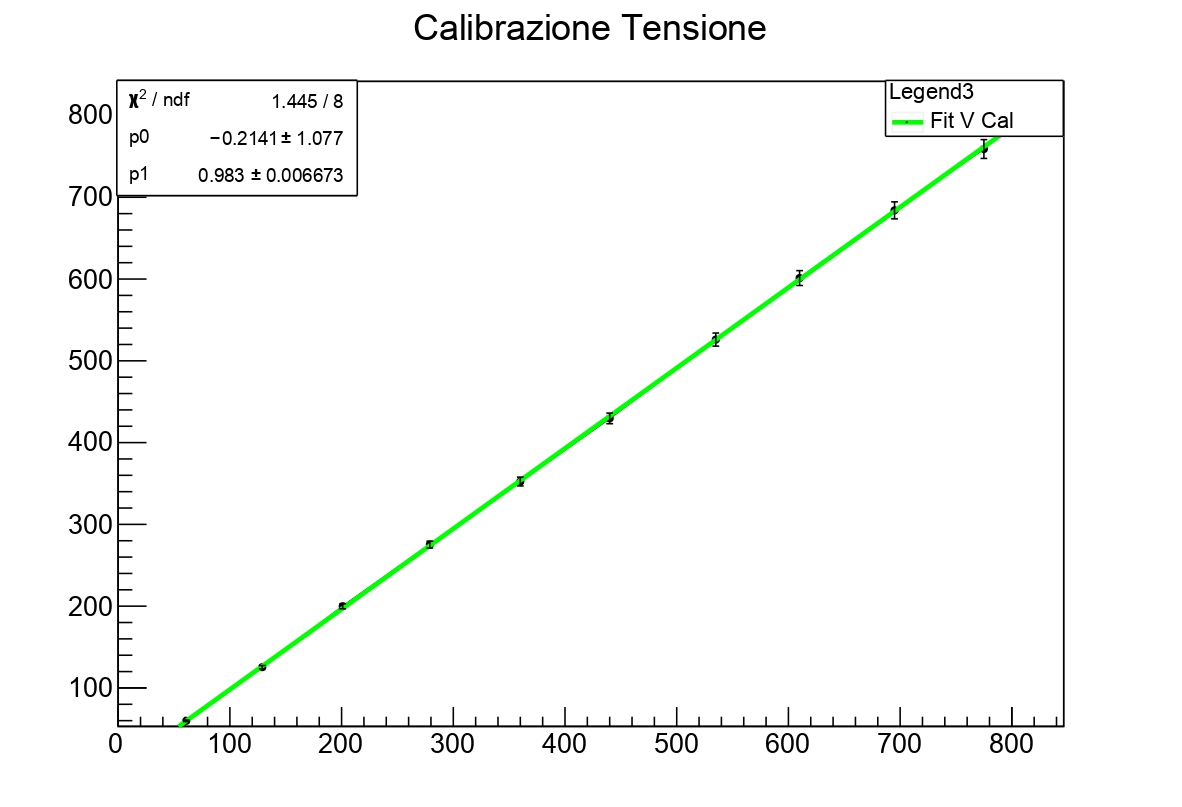
\includegraphics[scale=0.55]{Cal.jpg}
  \qquad
  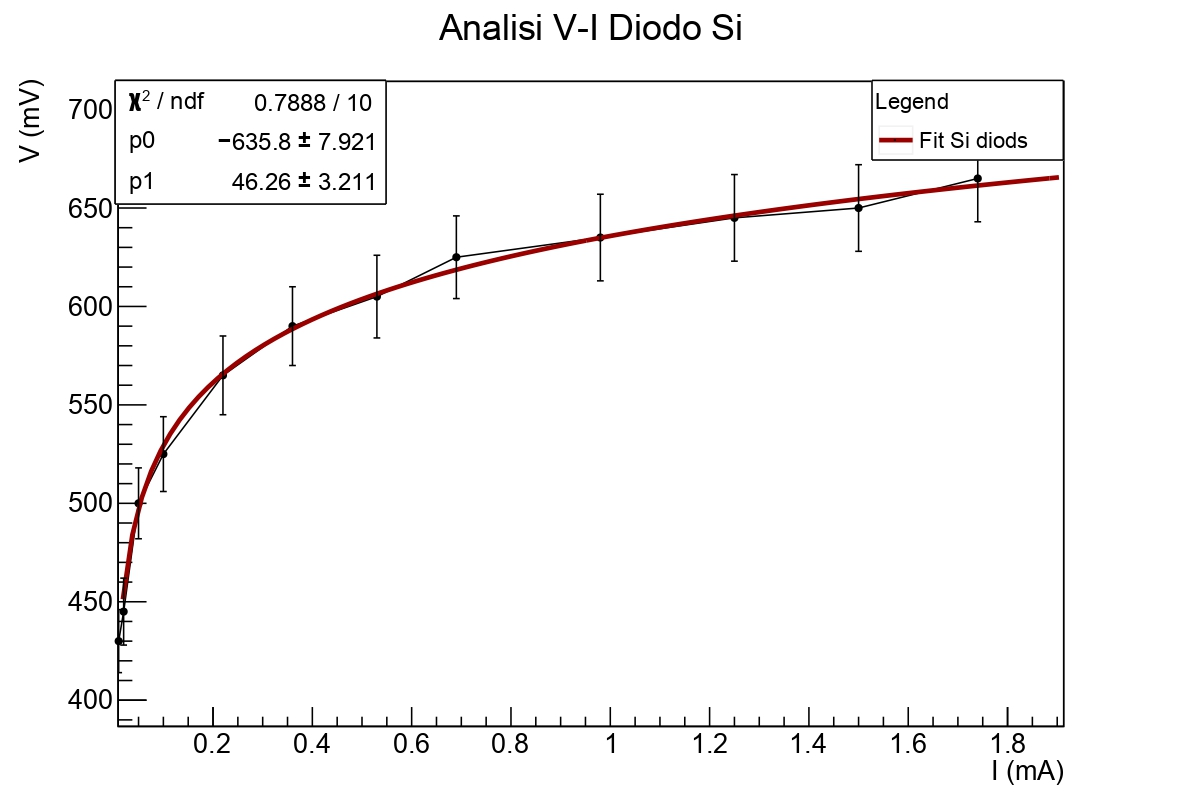
\includegraphics[scale=0.55]{SiLog.jpg}
  \qquad
  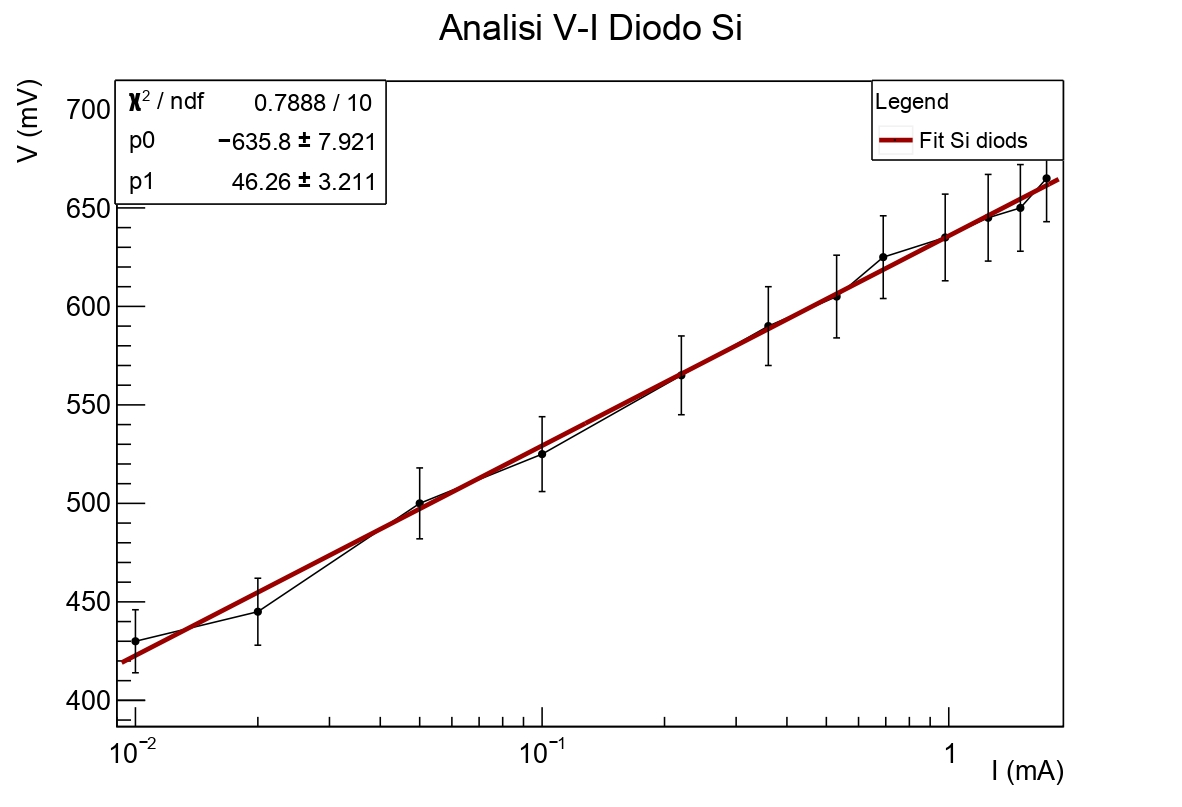
\includegraphics[scale=0.55]{SiLin.jpg}
  \qquad
  \caption{\textit{Grafici, dall'alto verso il basso, della retta di calibrazione, della caratteristica V-I del diodo al silicio e della stessa in scala semilogaritmica}}
\end{figure}

\begin{figure}[]
  \centering
  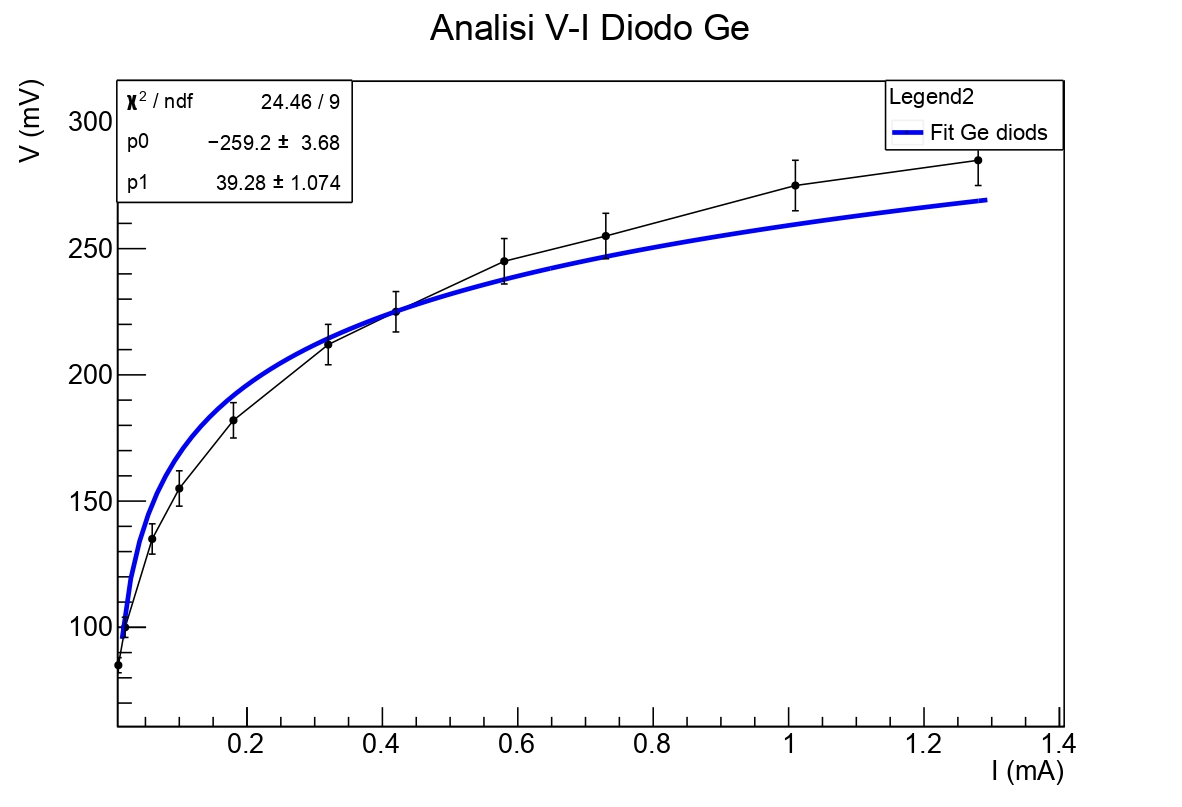
\includegraphics[scale=0.55]{GeLog.jpg}
  \qquad
  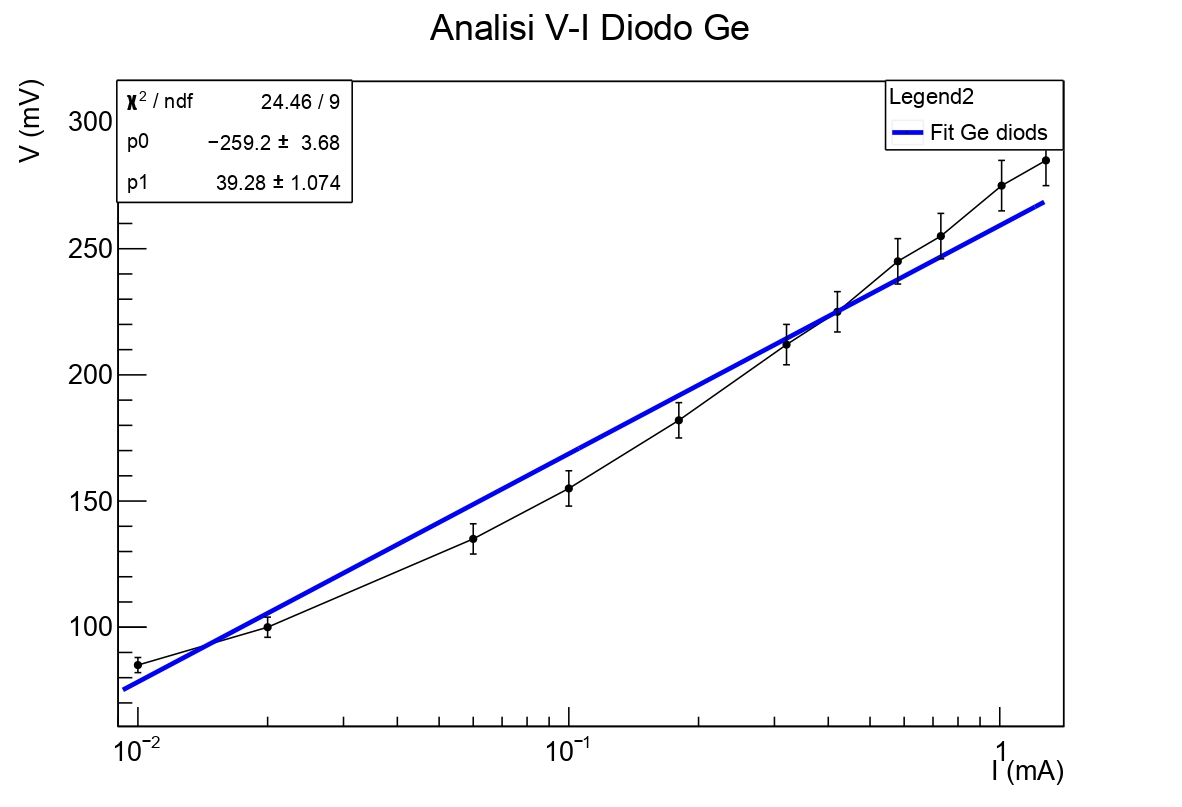
\includegraphics[scale=0.55]{GeLin.jpg}
  \qquad
  \caption{\textit{Grafici della caratteristica V-I del diodo al germanio e della stessa in scala semilogaritmica}}
\end{figure}




\section{Conclusioni}
Grazie ai grafici del fit ai dati sperimentali e ai valori calcolati di $I_0$ e $\eta V_T$ è stato possibile verificare,
almeno qualitativamente, la bontà delle previsioni teoriche sull'andamento della caratteristica V-I di diodi al silicio e al germanio.
Per migliorare i risultati si sarebbero potuti ad esempio effettuare un maggior numero di misure o migliorare l'accuratezza di quelle effettuate con l'oscilloscopio.






\end{document}
